\section{Data Durability, Consistency, and Reliability}
\label{sec:hotpot:xact}

Being distributed shared memory and distributed storage at the same time,
\dsnvm\ should ensure both correct shared memory accesses to \nvm\
and the persistence and reliability of in-\nvm\ data. 
\hotpot\ provides three guarantees: coherence among cached copies of in-\nvm\ data,
recovery from various types of failures into a consistent state,
and user data reliability and availability under concurrent failures.
Although each of these three properties have been explored before,
as far as we know, \hotpot\ is the first system that integrates all of them in one layer.
\hotpot\ also has the unique requirement of low software overhead to retain the performance benefit of \nvm.

\begin{itemize}
\item{\em Cache coherence.} 
In \hotpot, application processes on different nodes cache remote data in their local \nvm\ for fast accesses.
\hotpot\ provides two consistency levels across cached copies: 
{\em \ra}, multiple readers and single writer ({\em MRSW}) 
and {\em \rb}, multiple readers and multiple writers ({\em MRMW}).
MRMW allows multiple nodes to concurrently write and commit their local cached copies.
With \mrmw, there can be multiple versions of dirty data in the system (but still one committed version),
while \mrsw\ guarantees only one dirty version at any time.
An application can use different modes for different datasets,
but only one mode with the same dataset.
This design allows flexibility at the dataset granularity while guaranteeing correctness.
 
\item{\em Crash consistency.} 
Data storage applications usually have well-defined {\em consistent} states and need to move from 
one consistent state to another atomically.
When a crash happens, 
user data should be recovered to a consistent state ({\ie, \em crash consistency}). 
\hotpot\ guarantees crash consistency both within a single node ({\em \rcs}) and across distributed nodes ({\em \rcm}).
Note that crash consistency is different and orthogonal to cache
coherence in \ra\ and \rb. 

\item{\em Reliability and availability.} 
To ensure that user persistent data can sustain $N-1$ concurrent node failures, 
where $N$ is a user defined value, \hotpot\ guarantees that {\em \re}, once data has 
been committed, there are always $N$ copies of clean, committed data.

\end{itemize}

This section first discusses how \hotpot\ ensures crash consistency within a single node,
then presents the \mrmw\ and \mrsw\ modes and their atomic commit protocols, %and the optional group fetch protocol.
and ends with the discussion of \hotpot's recovery mechanisms under different crash scenarios.

\subsection{Single-Node Persistence and Consistency}
\label{sec:hotpot:singleconsistency}

Before ensuring user data's global reliability and consistency in \dsnvm,
\hotpot\ first needs to make sure that data on a single node can properly sustain power crashes (\rcs)~\cite{Memory-Persistency}.
\hotpot\ makes data persistent with the standard Intel persistent memory instructions~\cite{Delegated-persist},
\ie, \clflush, \mfence\ (note that we do not include the deprecated \pcommit\ instruction~\cite{Deprecating-PCOMMIT}).

After a node crashes, if its \nvm\ is still accessible, \hotpot\ will use the \nvm\ content to recover;
otherwise, \hotpot\ will use other nodes to reconstruct data on a new node (Section~\ref{sec:hotpot:recovery}).
For the former case, \hotpot\ needs to guarantee that user data in \dsnvm\ is in a consistent state after crash.
\hotpot\ also needs to ensure that its own metadata is persistent and is consistent with user data.

\hotpot\ maintains metadata on a local node to find user data and record their morphable states (\ie, \committed, \dirty, or \redundant).
Since these metadata are only used within a single node, \hotpot\ does not need to replicate them on other nodes.
\hotpot\ makes these metadata persistent at known locations in \nvm\ ---
a pre-allocated beginning area of \nvm.
\hotpot\ also uses metadata to record online state of the system (\eg, \on\ maintains a list of active \dn{}s that have a cached copy of data).
These metadata can be reconstructed by re-examining system states after recovery.
Thus, \hotpot\ does not make these metadata persistent.

{
\begin{figure}[t]
\begin{center}
\centerline{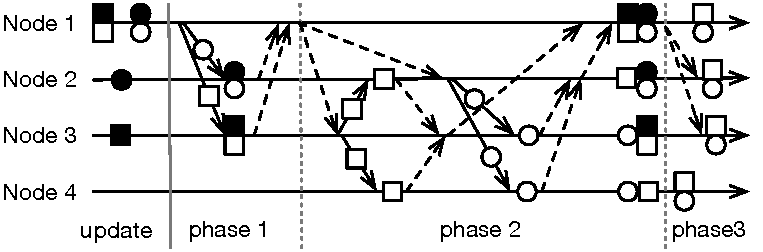
\includegraphics[width=\textwidth]{hotpot/Figures/commit.pdf}}
\caption[\mrmw\ Commit Example.]
{
\mrmw\ Commit Example.
Solid arrows represent data communication.
Dashed arrows represent metadata communication.
Node 1 (\xn) commit data to \on{}s at Node 2 and 3 with replication degree four.
Black shapes represent old committed states before the update
and white shapes represent new states.
}
\label{fig-mrmw}
\end{center}
\end{figure}
}

Similar to traditional file systems and databases, 
it is important to enforce {\em ordering} of metadata and data persistence
in order to recover to a consistent state.
For single-node non-commit operations (we defer the discussion of commit operations to Sections \ref{sec:hotpot:mrmw} and \ref{sec:hotpot:mrsw}), 
\hotpot\ uses a simple shadow-paging mechanism to ensure that the consistency of metadata and data.
Specifically, we associate each physical memory page with a metadata slot
and use a single 8-byte index value to locate both the physical page and its metadata.
When an application performs a memory store to a \committed\ page,
\hotpot\ allocates a new physical page, writes the new data to it, and writes the new metadata 
(\eg, the state of the new page) to the metadata slot associated with this physical page.
After making all the above data and metadata persistent, \hotpot\ changes the index
from pointing to the old \committed\ page to pointing to the new \dirty\ page.
Since most architectures support atomic 8-byte writes, this operation atomically moves the system to a new consistent state with both the new data and the new metadata.
%and \hotpot\ can always recover local data to a consistent state after crashes.

\subsection{\mrmw\ Mode}
\label{sec:hotpot:mrmw}
\hotpot\ supports two levels of concurrent shared-\nvm\ accesses and uses different protocols to commit data.
The \mrmw\ mode allows multiple concurrent versions of dirty, uncommitted data 
to support great parallelism.
\mrmw\ meets \rb, \rcm, and \re.

\mrmw\ uses a distributed atomic commit protocol at each commit point %(a user \commit\ call)
to make local updates globally visible, persistent, and replicated.
Since \mrmw\ supports concurrent commit operations 
and each commit operation can involve multiple remote \on{}s,
\hotpot\ needs to ensure that all the \on{}s reach consensus on the commit operation they serve. 
We designed a three-phase commit protocol for the \mrmw\ mode
based on traditional two-phase commit protocols~\cite{Samaras93,Gray78,Lampson81} but differs in that
\hotpot\ needs to ensure cache coherence, crash consistency, and data replication all in one protocol.
Figure~\ref{fig-mrmw} illustrates an example of \mrmw. 

{
\begin{figure}[th]
\begin{center}
\centerline{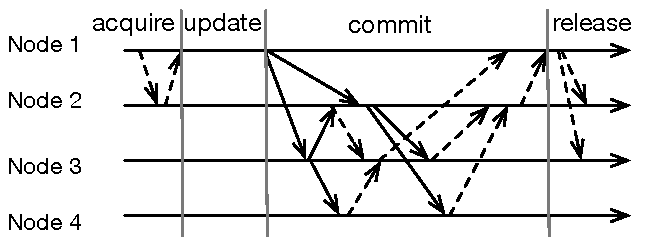
\includegraphics[width=\textwidth]{hotpot/Figures/mrsw.pdf}}
\caption[\mrsw\ Example.]
{
\mrsw\ Example.
Node 1 (\xn) first acquires write permission from Node 2 (\master)
before writing data.
It then commits the new data to \on{}s at Node 2 and 3 with replication degree four
and finally releases the write permission to \master.
}
\label{fig-mrsw}
\end{center}
\end{figure}
}


\noindent{\bf Commit phase 1.} 
When a node receives a \commitxact\ call (we call this node {\em \xn}), it checks if data specified in the \commitxact\ call is dirty
and commits only the dirty pages.
\xn\ persistently records the addresses of these dirty pages for recovery reasons (Section~\ref{sec:hotpot:recovery}).
\xn\ also assigns a unique ID ({\em \xactid}) for this \commitxact\ request and persistently records the \xactid\ and its state of starting phase 1. 
 
Afterwards, \xn\ sends the committing data to its \on{}s 
to prepare these \on{}s for the commit.
Each \on{} accepts the commit request if it has not accepted other commit request to the same pages,
and it stores the committing data in a {\em persistent redo log} in \nvm.
The \on\ also persistently records the \xactid\ and its state (\ie, completed phase 1) persistently.
The \on{} will block future commit requests to these data until the whole commit process finishes.
The \xn\ can proceed to phase 2 only when all \on{}s return successfully.

\noindent {\bf Commit phase 2.}
In commit phase 2, \hotpot\ makes the committing data persistent, 
coherent, and replicated.
This is the phase that \hotpot\ differs most from traditional distributed commit protocols.

\xn\ sends a command to all the involving \on{}s to indicate the beginning of phase 2.  
%This command indicates that the \on{}s can safely begin commit phase 2 and specifies the application's desired replication degree.  
Each \on{} then performs two tasks in one multicast operation (Section~\ref{sec:hotpot:network}): 
updating \dn{}s' cached copies of the committing data and making extra replicas.
\on\ looks up its metadata to find what \dn{}s have a cached copy.
If these \dn{}s alone cannot meet the replication degree, \on{} will choose new \dn{}s that do not have
a copy of the data and send the data to them.
%These \dn{}s mat have a \dirty, \committed, \redundant\ copy of the data, or they have no copy at all. 
%The \on{} does not differentiate these states and sends the updated data to all these \dn{}s. 

When a \dn{} receives the committing data from an \on,
it checks the state of its local data pages.
If a local page is in the \committed\ state or the \redundant\ state, 
the \dn\ will directly overwrite the local page with the received data.
In doing so, the \dn's cached \nvm\ data is updated.
If the local page is \dirty\  or if there is no corresponding local page,
the \dn\ allocates a new physical page and writes the new data to this page.
The new physical page will be in the \redundant\ state and will not affect the \dn's dirty data.
In this way, all \dn{}s that receive updated data from the \on\ will 
have a clean, committed copy, either in the \committed\ or the \redundant\ state.

After all \dn{}s have replied to the \on{} indicating that there are now $N$ copies of the committing data,
the \on\ commits data locally
by checkpointing (copying) data from the redo log to their home locations.
Unlike traditional databases and file systems that lazily checkpoint logged data, 
\hotpot\ checkpoints all committing data in this phase 
so that it can make the updated version of the data
visible to applications immediately, 
a requirement of shared-memory cache coherence.
During checkpointing, the \on{} will block both local and remote reads to the committing data
to prevent applications from reading intermediate, inconsistent data.

After the \xn\ receives successful replies from all the \on{}s, 
it deletes its old local data and moves to the new, committed version. 
At this point, the whole system has a coherent view of the new data
and has at least $N$ copies of it.
%The committing node can only proceed to phase 3 when all \on{}s returns successfully from phase 2.

\noindent {\bf Commit phase 3.}
In the last phase, the \xn\ informs all \on{}s that the \commitxact\ operation has succeeded.
The \on{}s then delete their redo logs.
%and make the new \committed\ data visible to applications.

\noindent {\bf Committing to a single \on\ and to local \on.}
When only one remote \on\ is involved in a \commitxact\ operation,
there is no need to coordinate multiple \on{}s
and \hotpot\ performs the above commit protocol in a single phase.

The \xn\ can also be the \on\ of committing data.
In this case, the \xn\ performs the \commitxact\ operation locally.
Since all local dirty pages are the COW of old \committed\ pages,
\xn\ already has an undo and a redo copy of the committing data
and does not need to create any other redo log as in remote \on's phase 1.

\subsection{MRSW Mode}
\label{sec:hotpot:mrsw}

The \mrsw\ mode allows only one writer to a \nvm\ page at a time
to trade parallelism for stronger consistency. 
%compared to the \mrmw\ mode.
\mrsw\ meets \ra, \rcm, and \re.

Traditional \mrsw\ protocols in DSM systems are usually invoked at every memory store
(\eg, to update cached read copies, to revoke current writer's write permission).
Unlike DSM systems, \dsnvm\ applications store and manage persistent data;
they do not need to ensure coherence on every memory store,
since they have well-defined points of when they want to start updating data and when they want to commit.
To avoid the cost of invoking coherence events on each memory store
while ensuring only one writer at a time, 
\hotpot\ uses an {\em \acquire} API for applications to indicate the data areas they want to update.
Afterwards, applications can update any date that they have acquired and use the \commitxact\ call to both 
commit updates and release corresponding data areas.
Figure~\ref{fig-mrsw} shows an example of \mrsw. % acquire, commit, and release process.

\noindent{\bf Acquire write permission.}
\hotpot\ uses a master node ({\em \master}) to maintain the active writer of each page. 
An \master\ can be one of the \hotpot\ node, the \cd, or a dedicated node.
%The \master\ maintains a simple hash table of the virtual page numbers of the data that is currently being written to.
When a node receives the \acquire\ call, it sends the virtual addresses of the data specified in the call to the \master.
If the \master\ finds that at least one of these addresses are currently being written to, 
it will reject the \acquire\ request and let the requesting node retry later.

\noindent{\bf Commit and release data.}
\mrsw's commit protocol is simpler and more efficient than \mrmw's,
since there is no concurrent commit operations to the same data in \mrsw\ (concurrent commit to different data pages is still allowed).
\mrsw\ combines phase 1 and phase 2 of the \mrmw\ commit protocol into a single phase 
where the \xn\ sends committing data to all \on{}s and all \on{}s commit data on their own.
%without the need to coordinate with other \on{}s.
Each \on\ individually handles commit in the same way as in the \mrmw\ mode, 
except that it does not need to coordinate with any other \on{}s or the \xn. 
\on\ directly proceeds to propagating data to \dn{}s after it has written its own redo log.

At the end of the commit process, the \xn\ informs the \on{}s to delete their redo logs (same as \mrmw\ commit phase 3)
and the \master\ to release the data pages.


